\documentclass[../probability-notes.tex]{subfiles}
\begin{document}
    %%%%%%%%%%%%%%%%%%%%%%%%%%%%%%%%%%%%%%%%%%%%%%%%%%%%%%%%%%%%%%%%%%%%%%%%%%%
    \section{Gamma Distribution}
    A random variable is said to have a Gamma distribution if for parameters $\lambda > 0, \alpha > 0$ it has the following probability distribution
    \begin{align*}
        p_{X}(x) = \begin{cases} 
            \frac{\lambda e^{-\lambda x} (\lambda x)^{\alpha - 1}}{\Gamma(\alpha)} &\mbox{if $x \geq 0$}\\
            0 &\mbox{otherwise}
        \end{cases}
    \end{align*}
    The denominator in the above fomula acts as nothing but a normalization constant and is defined as
    \begin{alignat*}{2}
        \Gamma (\alpha) &= \int_{0}^{\inf} \lambda e^{-\lambda x} (\lambda x)^{\alpha - 1}\\
        &= \int_{0}^{\inf} e^{-y} y^{\alpha - 1} dy &&\text{\;by letting $\lambda x = y$}\\
        &= (\alpha - 1) \int_{0}^{\inf} e^{-y} y^{\alpha - 2} dy &&\text{\;using integration by parts}\\
        &= (\alpha - 1) \Gamma (\alpha - 1)
    \end{alignat*}

    Note that at $\alpha = 1$, $\Gamma (1) = \int_{0}^{\inf} \lambda e^{-\lambda x} = 1$. Hence, if $\alpha$ is an integer, $\Gamma(\alpha) = \alpha !$ using the recursion relation derived above.\newline

    For a fixed $\lambda$, as the value of $\alpha$ becomes large, the distribution takes the form of a normal distribution.

    \begin{figure}[h]
    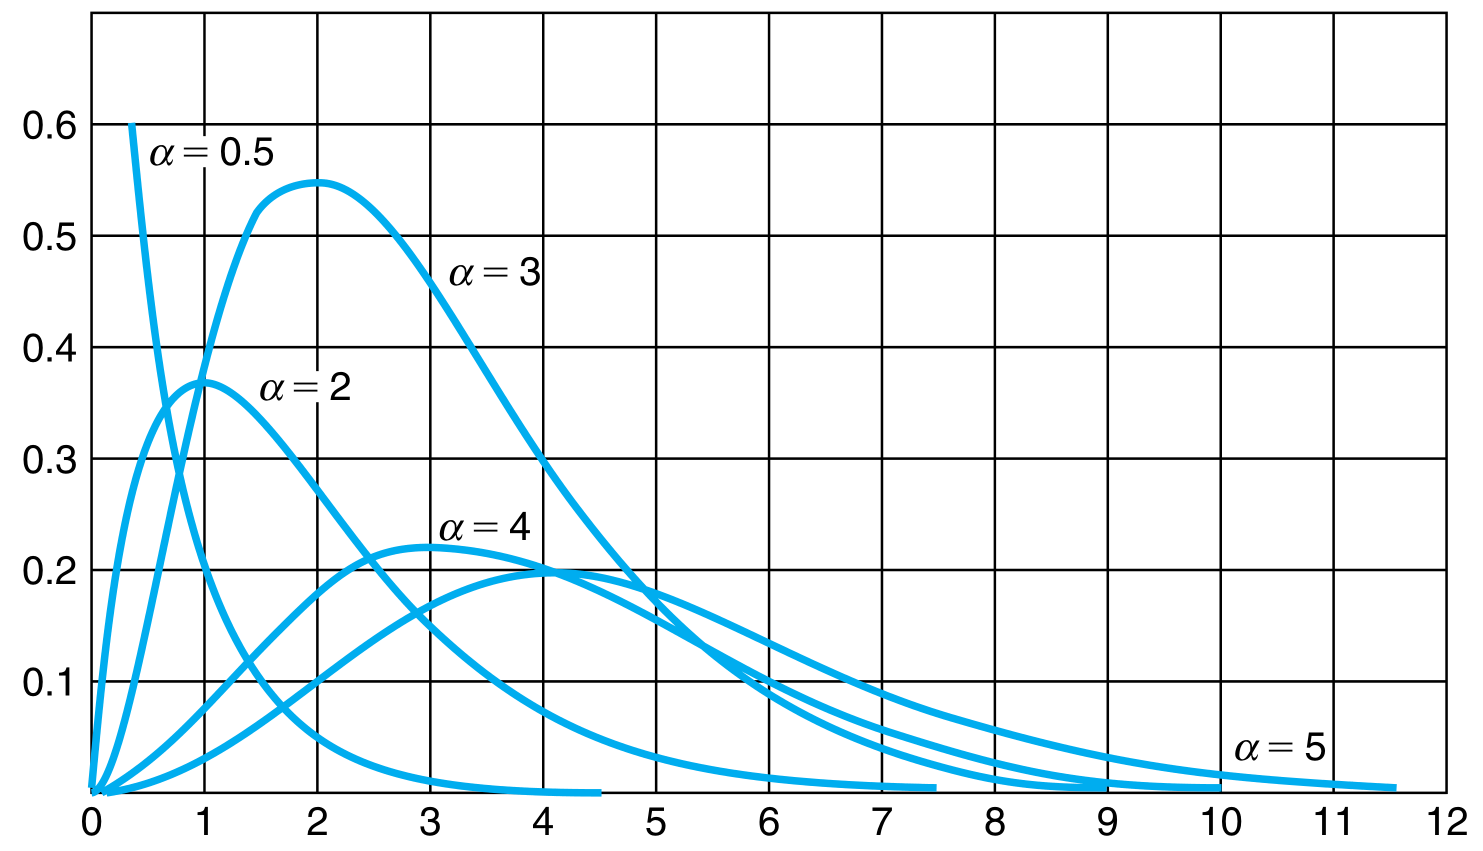
\includegraphics[scale=0.25]{gamma_1}
    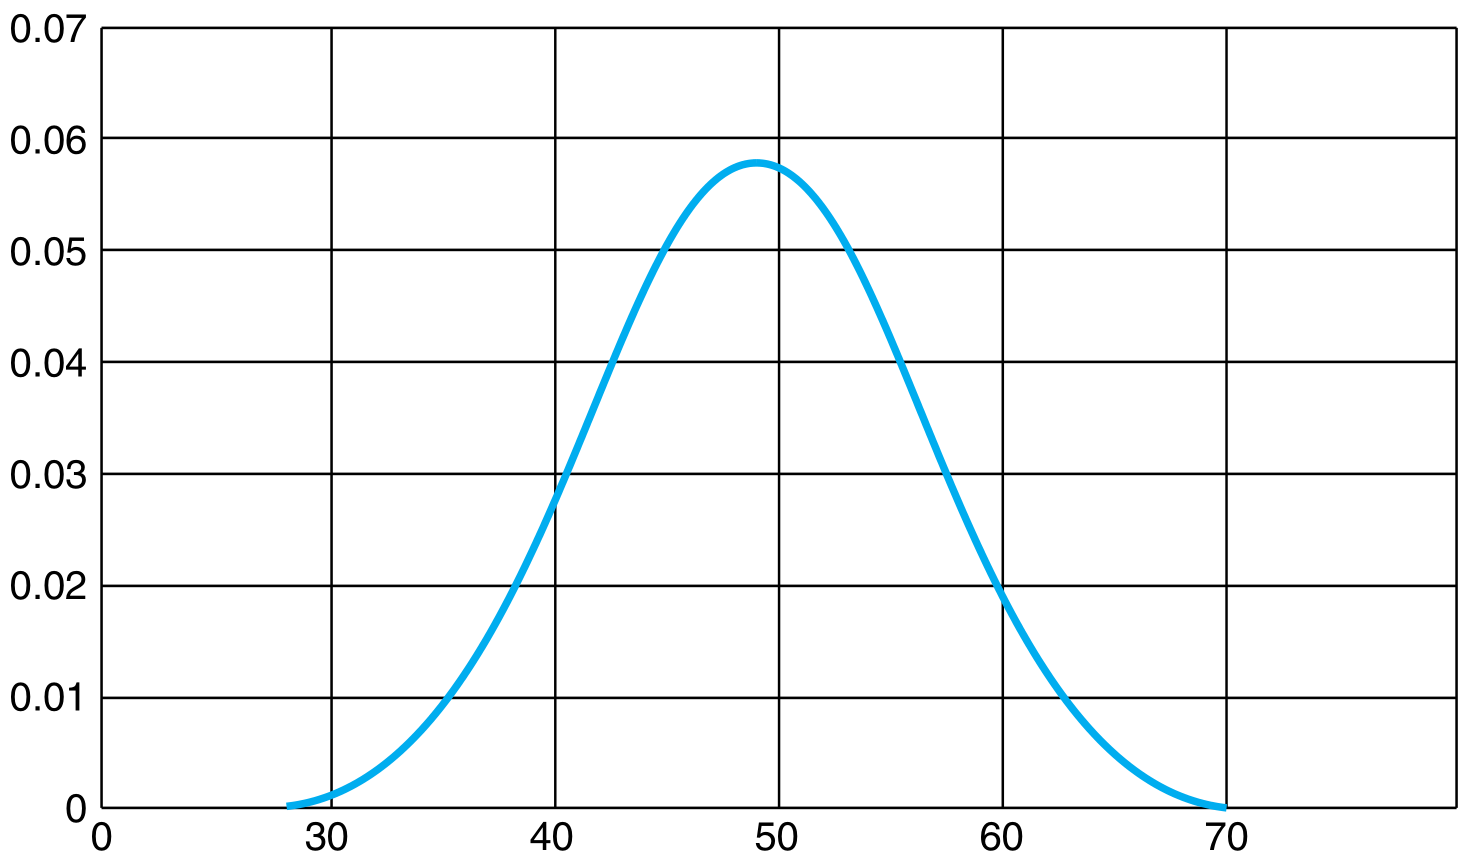
\includegraphics[scale=0.25]{gamma_2}
    \centering
    \caption{Gamma distribution for $\lambda = 1$ and different values of $\alpha$. The bottom figure shows the distribution for $\alpha = 50$.}
    \label{fig:gamma_1} %\ref{fig:gamma_1}
    \end{figure}

    %%%%%%%%%%%%%%%%%%%%%%%%%%%%%%%%%%%%%%%%%%%%%%%%%%%%%%%%%%%%%%%%%%%%%%%%%%%
    \subsection{Mean and Variance}
    Mean and variance are easily obtainable for this using the moment generating function. Recall
    \begin{align*}
        \phi(t) &= E[e^{tX}]\\
        \phi^{n}(t) &= E[X^{n}]
    \end{align*}

    For the current distribution,
    \begin{align*}
        \phi(t) &= \frac{\lambda^{\alpha}}{\Gamma(\alpha)} \int_{0}^{\inf} e^{tx} e^{-\lambda x} x^{\alpha - 1}\\
        &= (\frac{\lambda}{\lambda - t})^{\alpha}
    \end{align*}
    Differentiating,
    \begin{align*}
        \phi^{\prime}(t) &= \frac{\alpha \lambda^{\alpha}}{(\lambda - t)^{\alpha + 1}}\\
        \phi^{\prime \prime}(t) &= \frac{\alpha(\alpha + 1)\lambda^{\alpha}}{(\lambda - t)^{\alpha + 2}}
        \newline
        E[X] &= \phi^{\prime}(0)\\
        \Aboxed{E[X] &= \frac{\alpha}{\lambda}}\\
        Var(X) &= \phi^{\prime \prime}(0)\\
        \Aboxed{Var(X) &= \frac{\alpha}{\lambda^{2}}}
    \end{align*}

    %%%%%%%%%%%%%%%%%%%%%%%%%%%%%%%%%%%%%%%%%%%%%%%%%%%%%%%%%%%%%%%%%%%%%%%%%%%
    \subsection{Sum of Gamma Distributions}
    Let $X_{1}, X_{2}, \ldots, X_{n}$ be $n$ random variables that are gamma distributed with parameters \newline$(\alpha_{1}, \lambda), (\alpha_{2}, \lambda), \ldots, (\alpha_{n}, \lambda)$. Then the distribution of the sum of these random variables is itself a gamma distribution with the parameters $\alpha^{\prime} = \sum_{i=1}^{n} \alpha_{i}$ and $\lambda^{\prime} = \lambda$

\end{document}